%LTeX: language=de-DE
\chapter{Datenmodell}
Das Datenmodell (Common) wird von den Packages Frontend, Backend und Database importiert. Im Common Package wird der Vertrag erstellt, welche Daten zwischen den Packages ausgetauscht werden dürfen und wie diese Daten beschaffen sein müssen.
Die nachfolgende Abbildung [siehe Abb. \ref{fig: datamodel} auf S.~\pageref{fig: datamodel}] zeigt das Datenmodell der Applikation:
\begin{figure}[h]
    \centering
    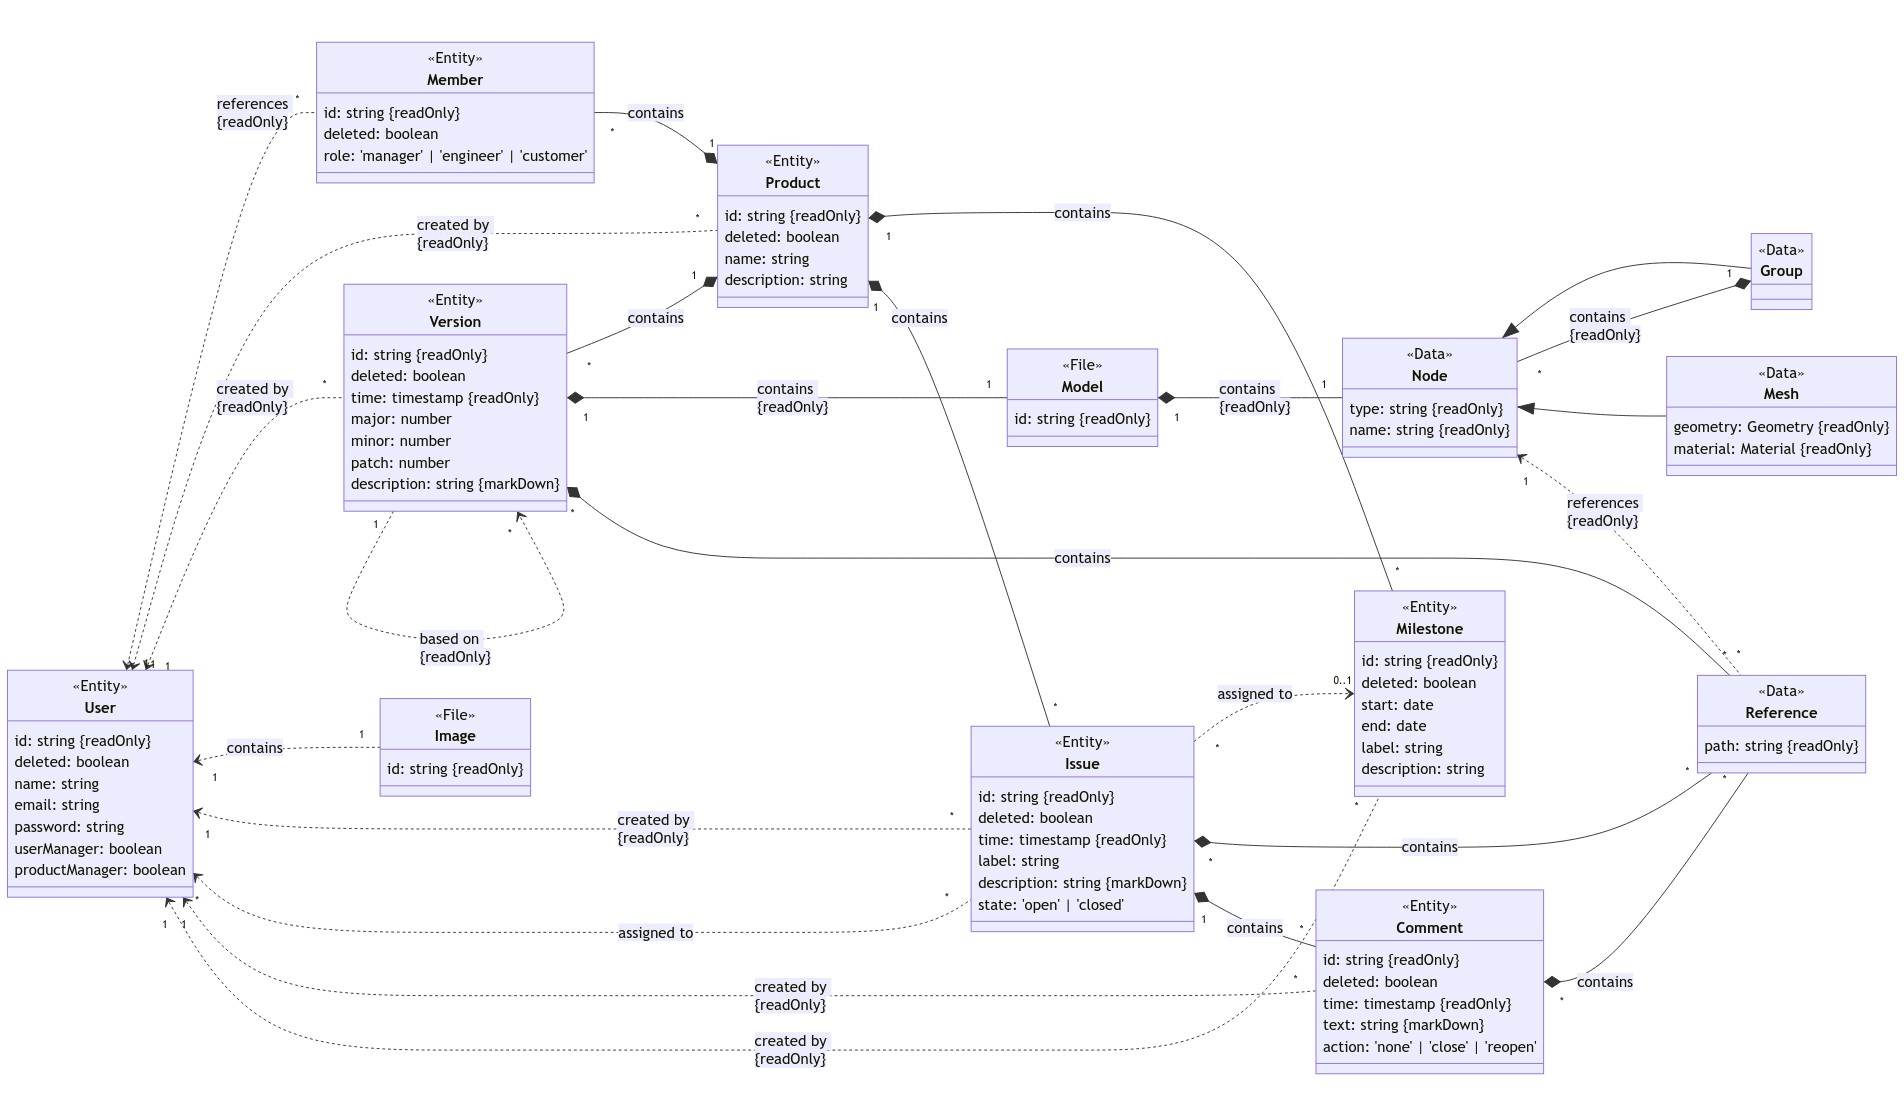
\includegraphics[width=1\textwidth]{datamodel.png}
    \caption{Datenmodell}
    \label{fig: datamodel}
\end{figure}

Die Implementierungen der Entities sind im Verzeichnis ''packages/common/src/data'' zu finden. Als Beispiel für die Implementierung wird, ein Ausschnitt vom Code für die ''ProduktEntity'' herangezogen [siehe Abb. \ref{fig: productdata} auf S.~\pageref{fig: productdata}]. In Zeile 1 wird das Modul für die Swagger-Dokumentation [siehe Abb. \ref{fig: swagger} auf S.~\pageref{fig: swagger}] eingebunden, welche alle Endpunkte der API übersichtlich auflistet. Mit dem Befehl ''@ApiProperty()'' werden dann die jeweiligen Einträge zur Swagger-Dokumentation\footnote{https://swagger.io}  hinzugefügt. Wie jedes Entity im Datenmodell, besteht auch das Product Entity aus drei Klassen: ''ProductUpdateData'', ''ProductAddData'', ''Product'', die hierarchisch aufeinander aufbauen. Sie definieren welche Daten später über die API geändert werden können, welche Daten beim Hinzufügen generiert werden und elementare Eigenschaften der Entity. 

\begin{figure}[h]
    \centering
    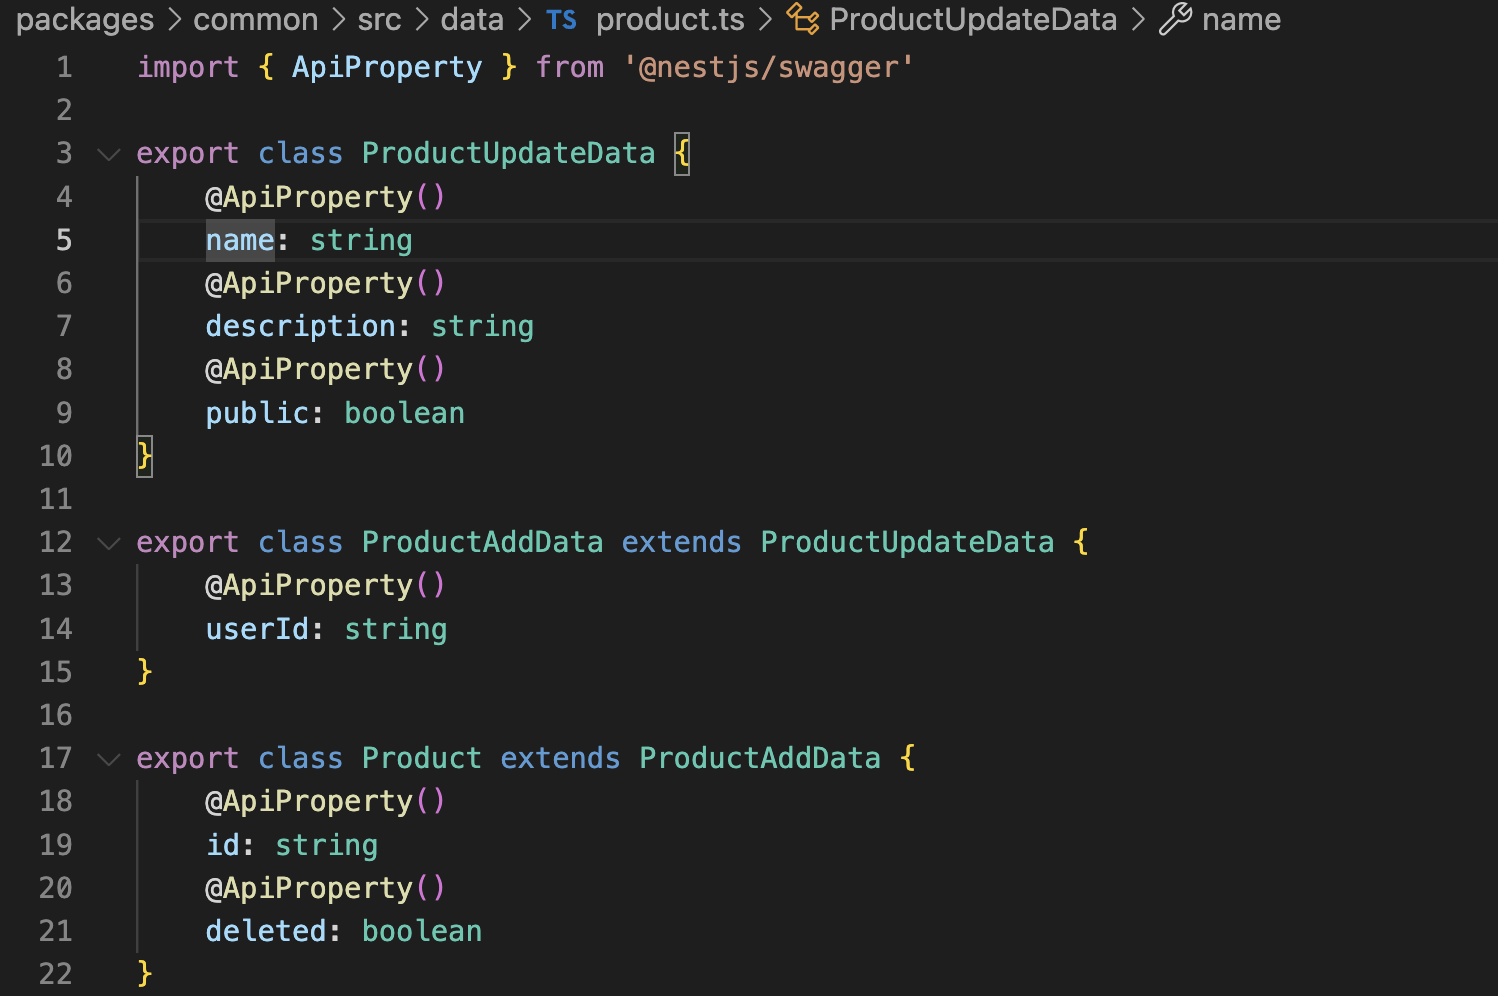
\includegraphics[width=1\textwidth]{productdata.png}
    \caption{Produkt Entity}
    \label{fig: productdata}
\end{figure}

\begin{figure}[h]
    \centering
    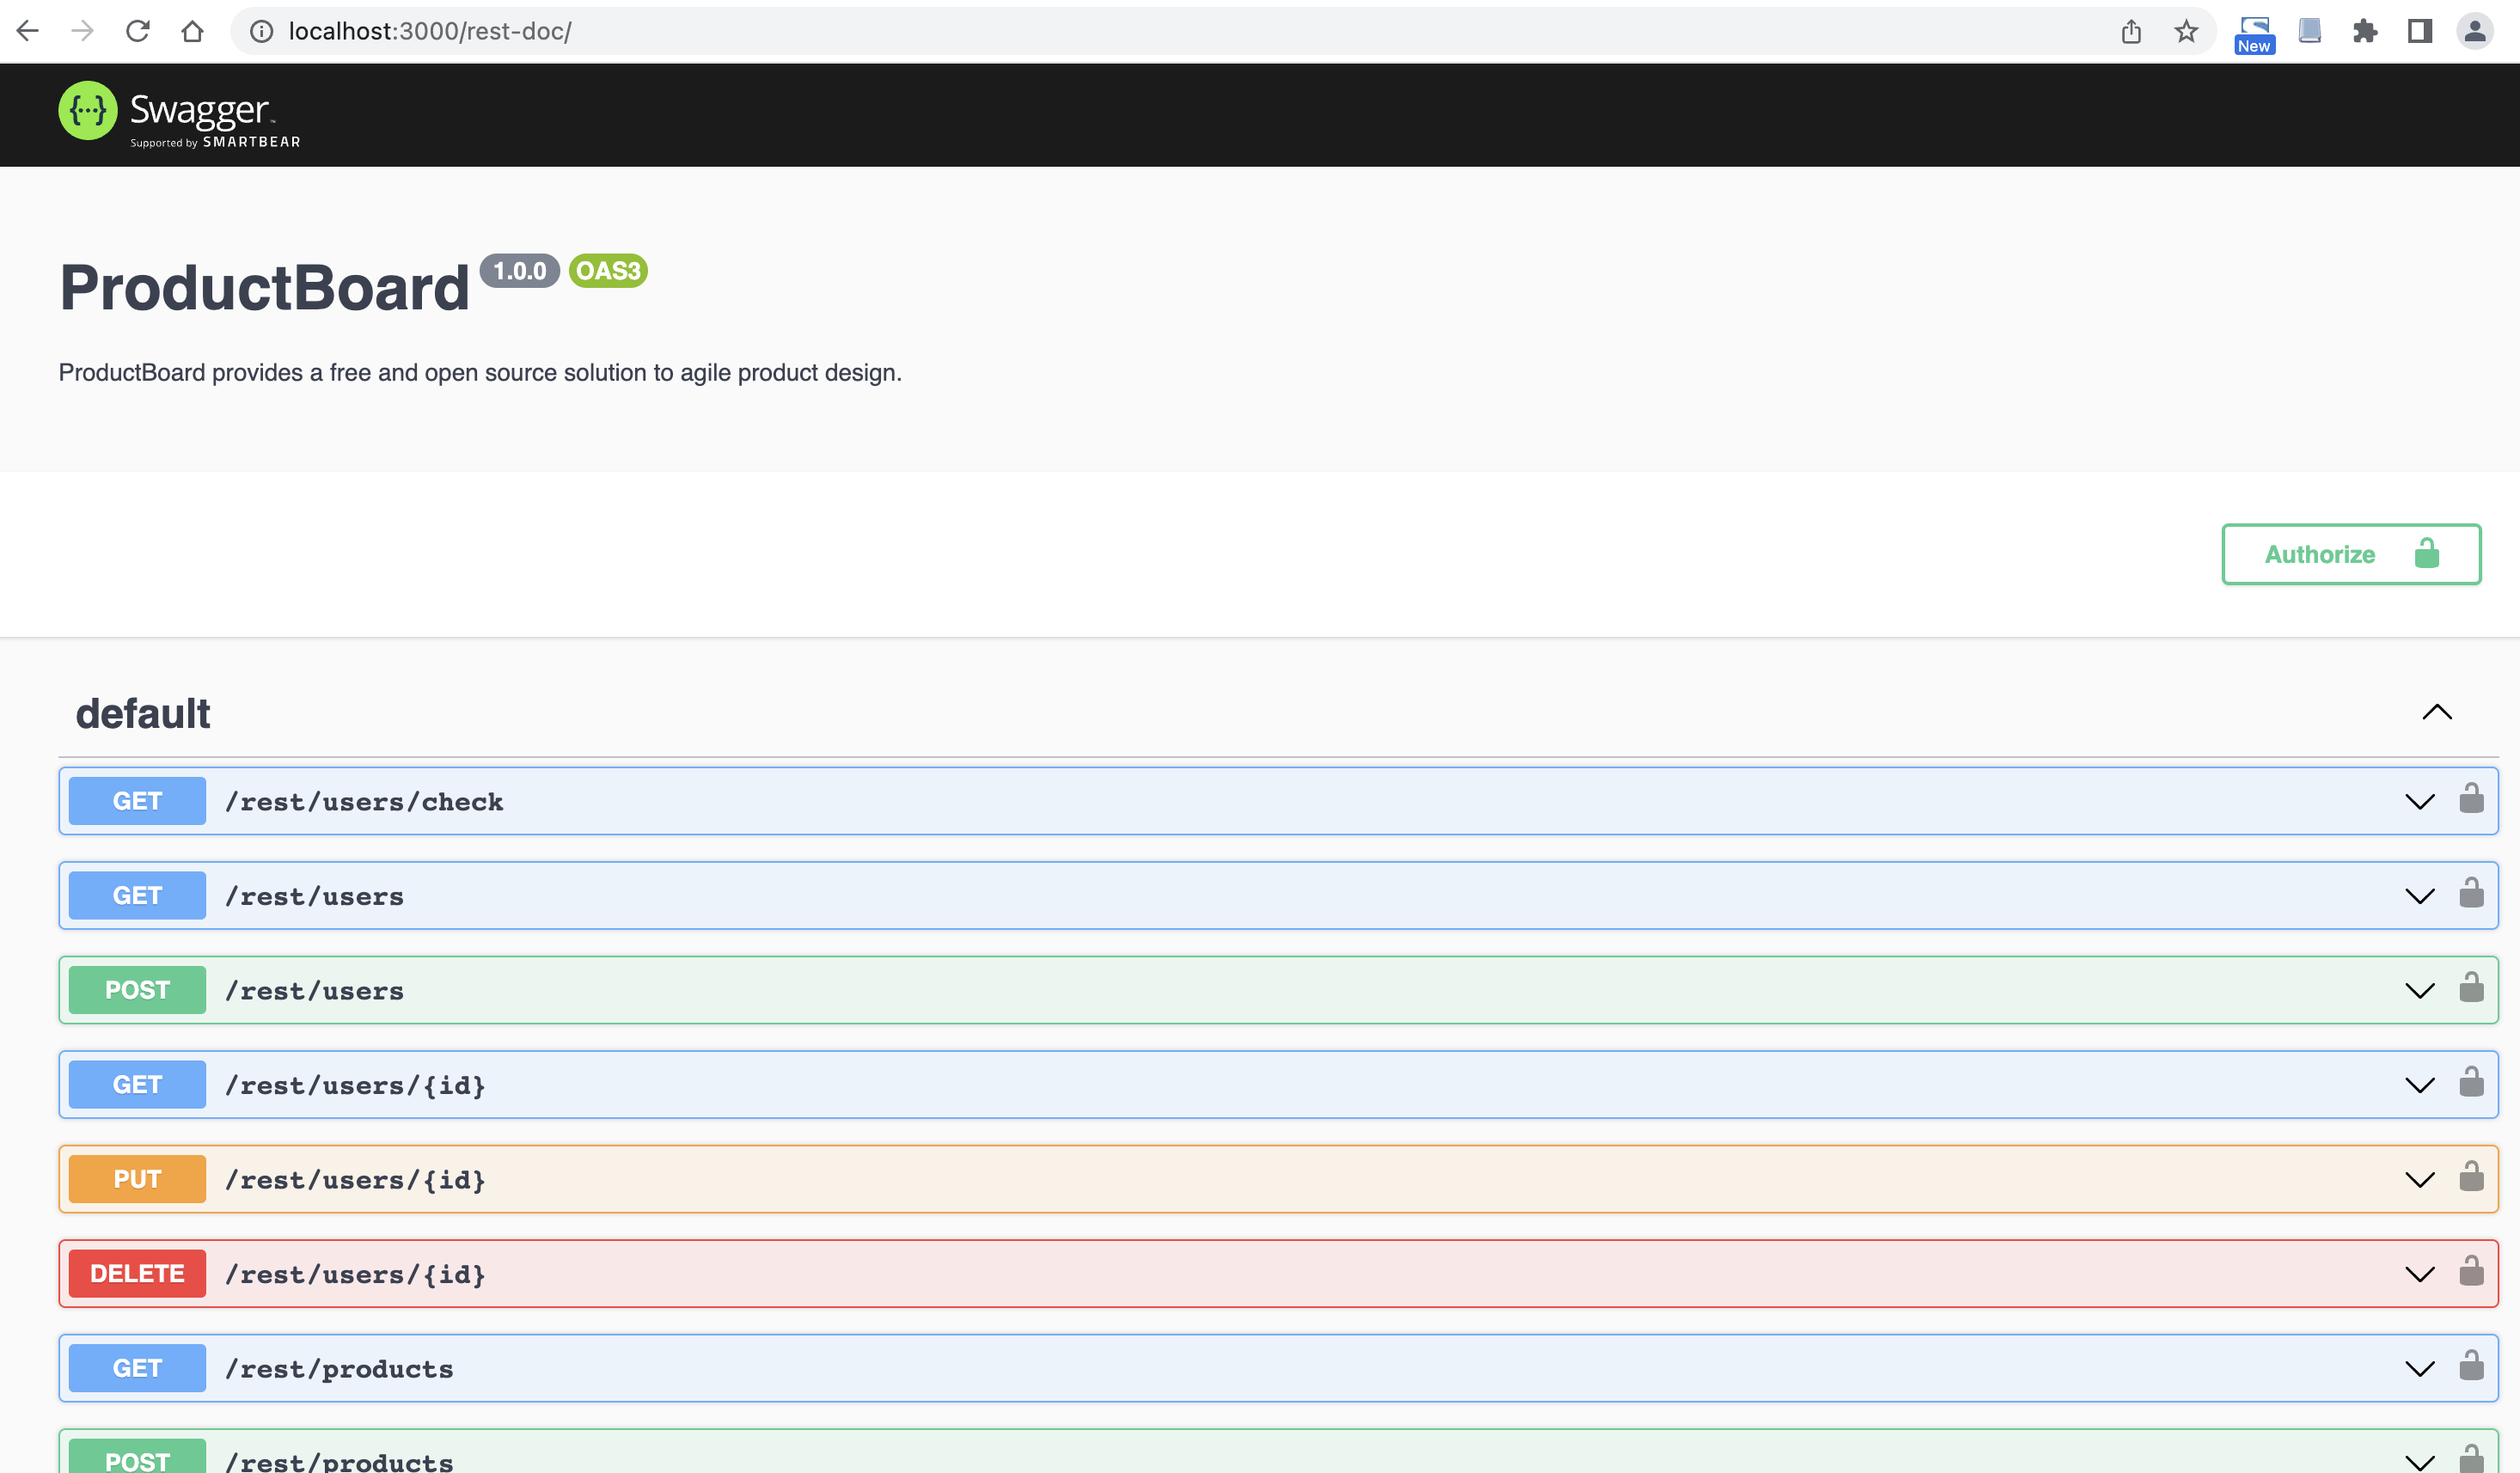
\includegraphics[width=1\textwidth]{swagger.png}
    \caption{Swagger Dokumentation}
    \label{fig: swagger}
\end{figure}